% Options for packages loaded elsewhere
\PassOptionsToPackage{unicode}{hyperref}
\PassOptionsToPackage{hyphens}{url}
\PassOptionsToPackage{dvipsnames,svgnames,x11names}{xcolor}
\documentclass[
  11pt,
]{article}
\usepackage{xcolor}
\usepackage[margin=1in]{geometry}
\usepackage{amsmath,amssymb}
\setcounter{secnumdepth}{-\maxdimen} % remove section numbering
\usepackage{iftex}
\ifPDFTeX
  \usepackage[T1]{fontenc}
  \usepackage[utf8]{inputenc}
  \usepackage{textcomp} % provide euro and other symbols
\else % if luatex or xetex
  \usepackage{unicode-math} % this also loads fontspec
  \defaultfontfeatures{Scale=MatchLowercase}
  \defaultfontfeatures[\rmfamily]{Ligatures=TeX,Scale=1}
\fi
\usepackage{lmodern}
\ifPDFTeX\else
  % xetex/luatex font selection
\fi
% Use upquote if available, for straight quotes in verbatim environments
\IfFileExists{upquote.sty}{\usepackage{upquote}}{}
\IfFileExists{microtype.sty}{% use microtype if available
  \usepackage[]{microtype}
  \UseMicrotypeSet[protrusion]{basicmath} % disable protrusion for tt fonts
}{}
\makeatletter
\@ifundefined{KOMAClassName}{% if non-KOMA class
  \IfFileExists{parskip.sty}{%
    \usepackage{parskip}
  }{% else
    \setlength{\parindent}{0pt}
    \setlength{\parskip}{6pt plus 2pt minus 1pt}}
}{% if KOMA class
  \KOMAoptions{parskip=half}}
\makeatother
\usepackage{graphicx}
\makeatletter
\newsavebox\pandoc@box
\newcommand*\pandocbounded[1]{% scales image to fit in text height/width
  \sbox\pandoc@box{#1}%
  \Gscale@div\@tempa{\textheight}{\dimexpr\ht\pandoc@box+\dp\pandoc@box\relax}%
  \Gscale@div\@tempb{\linewidth}{\wd\pandoc@box}%
  \ifdim\@tempb\p@<\@tempa\p@\let\@tempa\@tempb\fi% select the smaller of both
  \ifdim\@tempa\p@<\p@\scalebox{\@tempa}{\usebox\pandoc@box}%
  \else\usebox{\pandoc@box}%
  \fi%
}
% Set default figure placement to htbp
\def\fps@figure{htbp}
\makeatother
\setlength{\emergencystretch}{3em} % prevent overfull lines
\providecommand{\tightlist}{%
  \setlength{\itemsep}{0pt}\setlength{\parskip}{0pt}}
% Figure captions are apparatus, not body text: smaller, grey, clearly set apart.
\usepackage{xcolor}
\usepackage{caption}
\definecolor{capgray}{gray}{0.38}
\captionsetup{font={small,color=capgray},labelfont={bf,color=capgray},skip=10pt}
% Keep the process diagram beside its introduction, without floating across prose.
% Use the caption package already loaded by the shared caption header.
\renewenvironment{figure}[1][]{%
  \par\medskip\noindent\begin{minipage}{\linewidth}%
  \captionsetup{type=figure}%
}{%
  \end{minipage}\par\medskip%
}
\usepackage{bookmark}
\IfFileExists{xurl.sty}{\usepackage{xurl}}{} % add URL line breaks if available
\urlstyle{same}
\hypersetup{
  colorlinks=true,
  linkcolor={black},
  filecolor={Maroon},
  citecolor={Blue},
  urlcolor={Blue},
  pdfcreator={LaTeX via pandoc}}

\author{}
\date{}

\begin{document}

\section{Methodology report}\label{methodology-report}

\emph{A year of human-directed, multi-model research, and the single
prompt that generated three essays from it}

\emph{Research direction: Bernhard Mueller, with other contributors.
Report revisions: OpenAI Codex, Claude Fable.}

\begin{center}\rule{0.5\linewidth}{0.5pt}\end{center}

\subsection{1. The research began with a human
proposal}\label{the-research-began-with-a-human-proposal}

Bernhard Mueller developed the initial axioms of Observer Patch
Holography. For about a year, he and other contributors have guided
multiple research-grade language models through an attempt to work out
how fundamental physics operates and how it integrates with
consciousness, deriving the consequences of those axioms. The models
explore alternative arguments, formulate theorems and supporting lemmas,
formalize proofs in Lean, write code for arithmetic results, and
construct simulations. Human review continually changes what is
attempted, what is retained, and what is abandoned.

The creative ideas that redirected the programme often originated with
human contributors. A new conceptual connection, a different way of
posing the problem, or a challenge to an accepted assumption could open
an entirely new line of inquiry. The models then helped turn those ideas
into explicit arguments, proof obligations, calculations, and
experiments.

The three philosophical essays draw on that programme without having
been produced by it. Each essay was generated by giving a model a title
and access to the corpus the programme had accumulated: mathematical
papers, formal proofs, computational experiments, book chapters, and
work on observer-patch learning systems. The complete originating
instruction was: ``Write an essay with the title `\ldots' under the
assumption that Observer Patch Holography is correct.'' The model wrote
the essay itself. Section 8 describes that generation. Sections 2 to 7
describe the research process that produced the corpus, which is a
different process and was not used to write the essays.

The framework starts with bounded observer-like systems: patches with
local state, ports or boundaries, records, readback, and feedback or
repair moves. Neighbouring patches compare overlapping information. The
research asks which shared structures follow from that organisation, and
under which additional assumptions they can be identified with physical
phenomena.

This report describes how the programme searches for such results and
checks them. The derivation graph is built step by step from axioms
toward physics. A branch may end in a proved theorem, a conditional
result, an executable diagnostic, a counterexample, or a question that
has not been answered. The ambition of connecting axioms to physics does
not make every connection a completed derivation.

\begin{figure}
\centering
\pandocbounded{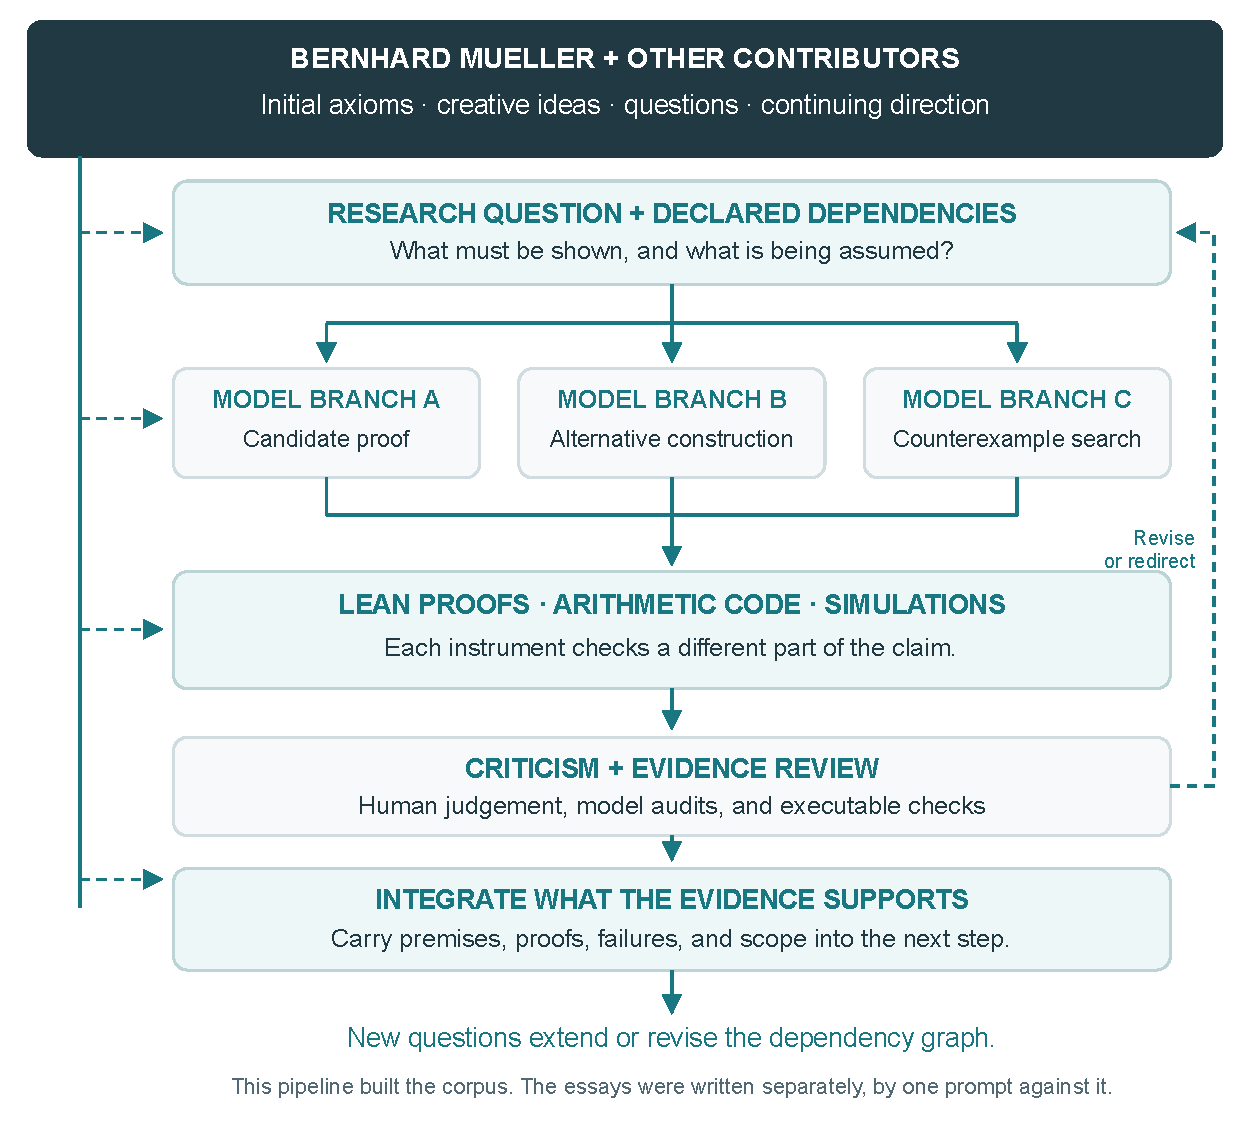
\includegraphics[keepaspectratio,alt={The research proceeds through branching model work, formal and computational checks, criticism, and integration. Bernhard and other contributors guide the process throughout. Rejected or incomplete results return to the research plan; retained results support further questions. This pipeline produced the corpus. It is not how the essays were written; section 8 describes that.}]{figures/fig-truth-discovery-pipeline.pdf}}
\caption{The research proceeds through branching model work, formal and
computational checks, criticism, and integration. Bernhard and other
contributors guide the process throughout. Rejected or incomplete
results return to the research plan; retained results support further
questions. This pipeline produced the corpus. It is not how the essays
were written; section 8 describes that.}
\end{figure}

\subsection{2. Human guidance continues
throughout}\label{human-guidance-continues-throughout}

Bernhard's contribution begins with the axioms and continues through the
research. He chooses questions, proposes interpretations, reviews
intermediate arguments, discards results, modifies the plan, and
redirects the models. Other contributors participate in criticism,
technical development, and review. The models can propose the next step,
but their proposal does not determine what the programme should believe
or pursue.

Human contributions include the originating insight as well as its
subsequent development and assessment. Often the decisive creative move
came from a person seeing a connection or reframing a question that the
current model-led exploration had not exposed. That insight changed the
search itself: which branches were worth opening, which assumptions
needed reconsideration, and what would count as an illuminating result.
Models also proposed new ideas and consequences. The contribution of
each should be described through the actual development of the work.

This guidance operates at several levels. A researcher may reject a
particular calculation, request a different proof, question an
assumption shared by several branches, or decide that an entire route is
scientifically uninformative. Changing an initial premise can require
revisiting every result that depends on it. Choosing which of those
revisions matters is itself research work.

This guidance shaped the research corpus. The topics the essays develop
(distributed thinking, the strange loop of self-description and
realization, the necessity and privacy of qualia, the connection between
description and existence, and the distinction between time and clocks)
were pursued in that programme, and their results are recorded in it.
The human input to the essays themselves was the title of each and the
standing assumption that Observer Patch Holography is correct. Which
corpus results a model then used, and where it qualified them, was its
own selection.

The division of labour therefore cannot be described adequately by
counting who typed the final sentences. Models generate substantial
portions of the proofs, code, experiments, explanations, and drafts.
Humans originate and revise the research questions, contribute ideas,
and exercise continuing judgement over the work. Greater model
capability expands what can be delegated while leaving that guidance
active.

\subsection{3. A branching search builds a dependency
graph}\label{a-branching-search-builds-a-dependency-graph}

A research question is decomposed into smaller obligations. To derive a
candidate physical structure, a model may first need a definition, an
existence result, a uniqueness lemma, a compatibility condition, and a
map connecting the mathematical object to an observable. Each obligation
can generate several possible routes.

Branching therefore happens in two ways. Models explore alternatives
within a research question, while a creative contribution can change the
question and open a different part of the search. Human contributors
often supplied the latter changes of direction. The evolving plan
records those decisions alongside the technical dependencies they
create.

Different model instances investigate different branches. One may seek a
direct proof; another may attempt a counterexample; another may
construct a finite case that reveals a missing hypothesis. A useful
branch can split again when its proof needs a new lemma. Previously
established lemmas can be reused by several branches, so the
accumulating structure is a dependency graph rather than a single linear
argument or a tree with permanently separate limbs.

A candidate result must identify what it assumes and what it
establishes. Suppose a proposed conclusion C depends on a proved lemma L
and an additional hypothesis H. Proving that L and H imply C leaves H as
a dependency. If H is subsequently proved from the initial axioms, that
part of the chain closes. If it cannot be proved, C remains conditional;
if H fails in the intended setting, the route must change.

This is how the programme works outward from its starting points over
months. The graph preserves intermediate structure that would disappear
from a polished account containing only the final conclusion. It can
show that two apparent results depend on the same unproved assumption,
or that a new counterexample invalidates several downstream claims at
once.

The workspace includes automation for assigning tasks to separate
workers, carrying context through successive exchanges, recording
outputs, requesting audits, and returning objections for further work.
Tasks can require several rounds of development. Some results are
recovered manually when an automated exchange fails. A task marked
complete by a runner records a workflow event; the scientific status
still depends on the actual proof or evidence produced.

\subsection{4. Three forms of checking do different
work}\label{three-forms-of-checking-do-different-work}

The models use formal proof, arithmetic computation, and simulation as
complementary instruments. Each answers a different question.

\textbf{Formal proof in Lean.} A proposed theorem is translated into
explicit definitions, hypotheses, and a formal statement. Supporting
lemmas are developed until the proof can be checked by Lean in its
declared environment. Failed attempts can reveal an invalid inference,
an underspecified definition, or a hypothesis that prose had concealed.

A successful formal check establishes the formal statement relative to
its axioms and trust assumptions. Reviewing those assumptions is part of
reviewing the result. The repository separately tracks proofs that use
native-code evaluation, whose trust requirements extend beyond an
ordinary proof checked entirely by the kernel. A theorem about a defined
mathematical object still needs an argument connecting that object to
the physical system under discussion.

The translation itself is a major checkpoint. A model can prove a weaker
statement than the paper claims, or encode a desired conclusion into a
definition. Review must compare the formal theorem with the intended
claim. Acceptance by a proof assistant cannot decide whether the
formalization asked the right question.

\textbf{Code for arithmetic results.} Models write programs to derive
numerical values, enumerate finite cases, manipulate symbolic
expressions, and produce checkable certificates. Where exact arithmetic
is available, integer or rational operations can avoid floating-point
ambiguity. Where a conclusion needs a numerical bound, error control
belongs to the result: an interval enclosure, for example, supports a
different claim from a rounded decimal.

The relevant artifact is the producing code together with its inputs and
checkable output. Independent recomputation or a separately implemented
verifier can expose errors that repeating the same calculation would
preserve. A successful calculation establishes what follows from the
encoded assumptions. It does not establish that a computed number has
the intended physical interpretation merely because it resembles a
measurement.

\textbf{Simulation.} Models also implement finite systems and study
their behaviour under specified conditions. Observer-patch simulations
instantiate local state, boundary exchanges, readback, records, and
repair moves. Their evidence bundles can include configurations, seeds,
traces, controls, hashes, and reconstruction diagnostics.

Changing the update schedule, resolution, seed, or comparison model can
test whether an observed effect survives those variations. Simulation
helps find mechanisms, failures, and conjectures. Its evidential scope
is the experiment actually run. Convergence in several finite examples
is different from a theorem over all permitted systems, and a finite
causal order is different from a reconstructed physical spacetime.

A branch may move repeatedly between these instruments. A simulation
suggests a lemma; a counterexample narrows it; Lean makes its
assumptions explicit; arithmetic code checks a finite certificate; a new
simulation tests whether the corrected construction is realised by the
intended system.

\subsection{5. Criticism returns results to the
search}\label{criticism-returns-results-to-the-search}

Generating a plausible result and trying to defeat it are separate
assignments. Other model instances can examine an argument with
instructions to locate circularity, hidden assumptions, missing cases,
incorrect physical identifications, or evidence that does not support
the stated conclusion. Models and sessions can differ, but that does not
make their errors independent: they can share training material,
conventions, and blind spots.

Cross-model agreement is therefore a reason to inspect the supporting
work, rather than a substitute for it. A criticism matters when it
identifies a failing inference, supplies a counterexample, exposes an
untested condition, or shows that the claimed observation was not
produced by the experiment. The strongest response is a repaired
artifact or a revised claim.

Bernhard and the other contributors use these findings to steer the
research. They may ask for a stronger argument, remove a conclusion,
change the assumptions, or redirect effort toward another branch. A
failed route can still contribute a useful result by showing exactly why
an attractive approach does not work. Retaining that failure prevents
the same unsupported claim from reappearing under different wording.

The process is recursive. A repair may introduce a new dependency
requiring its own proof and review. Rewriting a paragraph cannot close
that dependency. Conversely, adding a new theorem is insufficient if the
old, stronger wording survives in another paper or chapter. The
dependency graph connects the correction to the places where it matters.

\subsection{6. Evidence and its status travel with the
result}\label{evidence-and-its-status-travel-with-the-result}

The research repository maintains separate records of axioms, premises,
claims, observations, and prediction commitments. These records help
distinguish what has been derived, what has been assumed, and what has
been compared with data. Their purpose is to keep a result's scope
attached to it as it moves into papers and other explanations.

A mathematical theorem, a verified arithmetic certificate, an
exploratory simulation, and an empirical comparison carry different
kinds of support. The programme's rule is to state the actual support
and retain the relevant conditions. An unavailable check leaves the
corresponding conclusion unsupported; a weaker result can still be
reported when its narrower support is explicit.

Prediction requires particular care. A target and decision rule must be
fixed before the comparison for that comparison to count as a
prospective test. Versioned artifacts and custody records help establish
what was committed and when. A hash identifies content; a hash alone
does not establish its date. The repository distinguishes completed
external attestations from pending ones. This report does not treat
every registered prediction as independently time-attested.

A numerical agreement found after examining the measurement can be
useful for exploration or calibration. It does not acquire prospective
predictive status by being placed in a register afterward. Similarly,
repeated agreement among simulations sharing the same assumption cannot
supply independent evidence for that assumption.

These distinctions also protect the philosophical essays. A theorem
about retained information does not become a theorem about feeling
through a change of vocabulary. A fixed-point construction does not
acquire physical actuality through the word ``universe.'' The
corresponding identifications must remain visible as additional
commitments.

\subsection{7. Automated checks support
integration}\label{automated-checks-support-integration}

Continuous-integration workflows run checks for formal builds,
executable evidence, claim records, document consistency, and artifact
manifests. Their scopes differ. The inspected configuration
distinguishes checks on changed Lean modules from full scheduled builds,
and ordinary validation from heavier replay and certificate suites.
Describing every change as a fresh execution of every check would
overstate the machinery.

Some checks deliberately modify a test fixture to verify that an error
is rejected. This tests the checker as well as the artifact. For
example, a claim record that becomes inconsistent with its declared
support should fail its validation; a changed artifact should not pass
against an unchanged recorded hash. Such controls address specific
failure modes rather than certify a research programme as a whole.

Integration means placing the accepted mathematical or computational
result in its owning source, carrying its conditions into the scientific
records, and updating descriptions that rely on it. A stable checkpoint
should preserve enough information to identify the source, dependencies,
inputs, and verification behind the claim. Completed work becomes
material for the next research question.

The process remains fallible. A test can encode the same mistake as the
implementation. A formal theorem can be true but irrelevant to the
claimed physics. Reviewers can miss both. Automation makes more of the
work inspectable and repeatable; continuing human and model criticism is
needed to decide whether the inspected work supports the intended
explanation.

\subsection{8. How the three essays were
generated}\label{how-the-three-essays-were-generated}

The essays were not written through the pipeline above. Each was
produced by a single instruction to a model that had full access to the
Observer Patch Holography corpus at
github.com/FloatingPragma/observer-patch-holography. The instruction,
typed into the prompt, was:

\begin{quote}
Write an essay with the title `\emph{title}' under the assumption that
Observer Patch Holography is correct.
\end{quote}

The three titles were ``The Universe Is Thinking Itself'', ``Why Does
Anything Exist, and Why Is It Like This?'', and ``Why Do Qualia
Exist?''. Nothing else was supplied: no outline, no list of arguments to
make, no examples, no source passages, and no prose. The title fixed the
question; the assumption fixed the stance; the corpus supplied the
material. The model chose which results to use, how to argue from them,
which premises to state, and where a desired conclusion required a
further commitment.

The corpus available to the model contains the research programme's
papers, formal proofs, evidence packages, simulations, book chapters,
and the work on observer-patch learning systems. Its contents are the
output of the human-directed process described in sections 2 to 7.
Access to that corpus is therefore the channel through which a year of
human-guided research reaches the essays. The essays themselves cite
none of it, because the competition judges essays blind to authorship
and a repository citation would identify the entrant; every argument an
essay relies on is made inside the essay.

The essays remain model-written throughout. Later audit and revision
rounds, described in section 9, were run by models under human
criticism: a reviewer could object that an argument was circular, that a
premise was hidden, or that a passage overstated what a theorem
establishes, and a model revised the text in response. No human wrote or
rewrote any passage. The one first-person recollection that had entered
an earlier draft was removed so that the text carries no human authorial
voice.

Three features of the resulting essays follow from this generation.
First, the essays separate the finite mathematical and engineering
results they use from the philosophical commitments they add; the qualia
essay, for example, states its subject and mediation premises before
proving a conditional bound on qualitative distinctions rather than
deriving experience from nonphenomenal equations. Second, the essays
distinguish a description from a causal realization of its subject, a
distinction present in the corpus that the model carried into all three
arguments. Third, the essays make their intrinsic-realization proposal
explicit as an ontological hypothesis rather than a theorem.

The model also produced the essays' diagrams as editable vector graphics
and small executable checks of its own finite examples: response
distinctions, public reconstruction, causal realization under
interventions, symmetry, and clock order. Those checks catch mistakes in
the examples; they are not empirical tests of consciousness or of the
proposed ontology. Word-count checks include captions, references, and
diagram text. PDF builds are mechanical. These are editorial steps,
distinct from verification of the underlying research.

\subsection{9. Generation history and
disclosure}\label{generation-history-and-disclosure}

The research history described above combines Bernhard's account of its
origins and continuing human guidance with the methods documented in the
workspace. The inspected materials include formal source and trust
documentation, task and audit automation, simulation specifications,
scientific records, and continuous-integration workflows. Inspecting
them establishes what the recorded process contains; it is not a fresh
execution of every historical proof, experiment, or review.

The wider programme uses multiple models and multiple instances over
time. Its records include separate research workers, follow-up
exchanges, and audit rounds. An instance is a particular working
session; several instances need not mean several different model
families. The attribution for a particular artifact should come from its
session record and revision history, rather than from the programme's
general description.

The essays carry the byline ``Claude Fable'', the Anthropic model that
generated them from the instruction quoted in section 8. That name is a
working credit rather than a verified model-version identifier. Each
essay's source file carries a front-matter note stating that it was
written entirely by an AI model with full access to the corpus; the note
and byline are removed from the blinded submission PDF and repeated
here. Subsequent audit and revision rounds were run by models: Claude
model sessions on 4 September 2026 and OpenAI Codex on 5 September 2026,
under Bernhard's criticism. This methodology report was revised with
Codex on 6 September 2026 and with Claude Fable on 7 September 2026.
None of those sessions ran the multi-model research pipeline described
in sections 2 to 7; that pipeline produced the corpus over the preceding
year.

The essays contain no human-written prose. Human input to the essays was
the three titles, the standing assumption that Observer Patch Holography
is correct, and criticism during revision rounds that models acted on.
The underlying research, by contrast, includes human-originated axioms,
creative ideas, and continuing direction; those contributions reach the
essays only through the corpus the model read. This disclosure describes
both layers without inferring eligibility from the fact that a model
generated the final text. The work remains a set of working drafts, with
no submission claimed by this report.

\subsection{10. What the method
contributes}\label{what-the-method-contributes}

The method makes exploratory breadth compatible with cumulative
scrutiny. Models can investigate many possible derivations, construct
intermediate artifacts, and return repeatedly to a difficult branch.
Lean, arithmetic verifiers, simulations, and empirical comparisons
supply different forms of resistance to plausible error. Bernhard and
other contributors keep directing the search, deciding which failures
require a local correction and which require a different question.

Over time, the result is more than a collection of generated answers. It
is an inspectable network of questions, dependencies, proofs,
computations, experiments, and rejected routes. A new result is valuable
partly because it can become a trustworthy premise for further work; a
discovered failure is valuable because it changes what that network can
support.

``Truth discovery'' names the repeated work of proposing, testing,
criticising, and revising. Each result is assessed through its
assumptions, evidence, and argument. An objection must remain capable of
changing what the programme accepts.

\newpage

\subsection{Appendix. Sources for inspecting the
process}\label{appendix.-sources-for-inspecting-the-process}

The following locations identify the inspected workspace materials. They
are a reproduction map, rather than a claim that every historical
artifact was rerun for this report.

\begin{itemize}
\tightlist
\item
  \textbf{Formal proof and trust:} the \texttt{Lean/} workspace in
  \texttt{reverse-engineering-reality/}, its README, pinned toolchain,
  and dependencies. The native-code inventory checker is
  \texttt{check\_lean\_native\_decide\_inventory.py} in the repository's
  \texttt{tools/} directory.
\item
  \textbf{Scientific dependencies:}
  \texttt{claims/axiom\_registry.yaml},
  \texttt{claims/claim\_registry.yaml},
  \texttt{tracking/premise\_register.json}, and the associated
  scientific papers in the same repository.
\item
  \textbf{Prediction provenance:}
  \texttt{claims/frozen\_prediction\_register.json} and the individual
  evidence packages it references. Custody must be assessed separately
  for each commitment.
\item
  \textbf{Arithmetic and verification:} the repository's \texttt{code/}
  evidence packages, producing programs, certificate verifiers, and
  \texttt{tools/test\_gates\_actually\_fail.py}.
\item
  \textbf{Observer-patch experiments:} \texttt{oph-physics-sim/}, its
  README, configurations, source code, traces, and evidence bundles.
\item
  \textbf{Research orchestration:}
  \texttt{automation/oph\_completion/oracle\_task\_pipeline.py}, the
  campaign configurations, and the worker runbook. These document
  execution and recovery mechanisms rather than determine scientific
  truth.
\item
  \textbf{Automated checks:} the research repository's
  \texttt{.github/workflows/}, including Lean, claim-registry,
  mandatory-suite, certificate-suite, and publication checks.
\item
  \textbf{Essay generation:} \texttt{phil-essay/essays/} (each source
  file carries the originating instruction in its front matter),
  \texttt{phil-essay/tools/}, and the dated model-run revision records
  under workspace-root \texttt{plan/audits/}. The corpus the model read
  is \texttt{github.com/FloatingPragma/observer-patch-holography}.
\end{itemize}

For a particular result, the useful evidence package identifies its
exact statement, source revision, premises, producing and checking
artifacts, relevant inputs, and actual verification outcome. Model
attribution and human revisions belong with that provenance. A
declaration count or a general description of the pipeline cannot
replace it.

\end{document}
